\documentclass{standalone}
\usepackage{tikz}
\usetikzlibrary{patterns, positioning}

\begin{document}
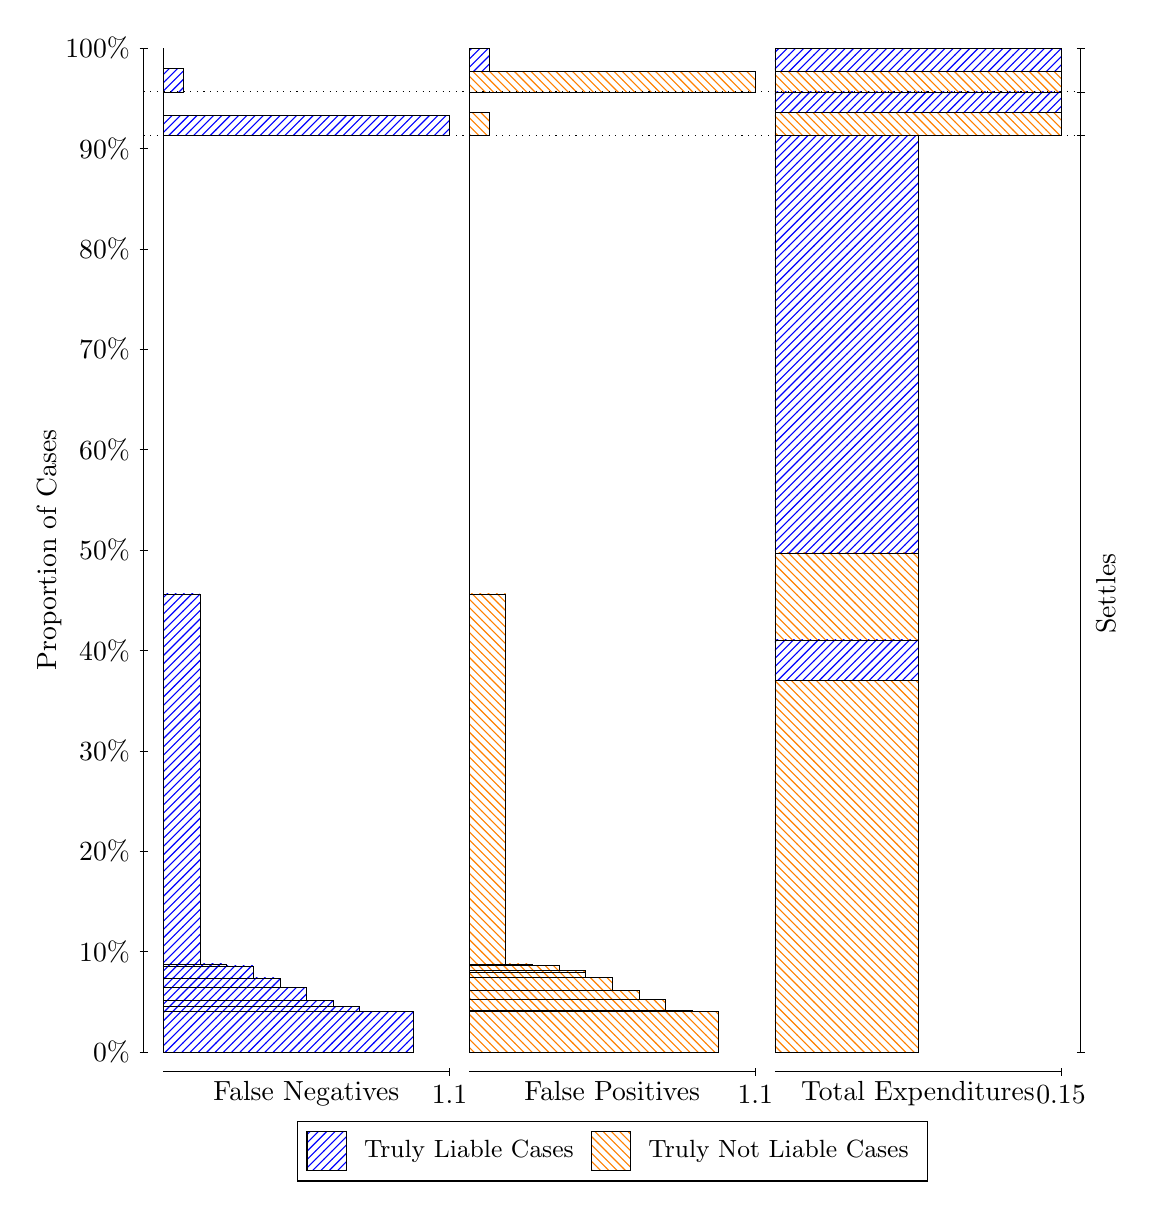
\begin{tikzpicture}
\draw[black, very thin] (1.5,1.75) -- (1.5,14.5);
\node[rotate=90, anchor=center] at (0.3, 8.125) {Proportion of Cases};
\draw[black, very thin] (1.45,1.75) -- (1.55,1.75);
\node[anchor=east] at (1.45, 1.75) {0\%};
\draw[black, very thin] (1.45,3.025) -- (1.55,3.025);
\node[anchor=east] at (1.45, 3.025) {10\%};
\draw[black, very thin] (1.45,4.3) -- (1.55,4.3);
\node[anchor=east] at (1.45, 4.3) {20\%};
\draw[black, very thin] (1.45,5.575) -- (1.55,5.575);
\node[anchor=east] at (1.45, 5.575) {30\%};
\draw[black, very thin] (1.45,6.85) -- (1.55,6.85);
\node[anchor=east] at (1.45, 6.85) {40\%};
\draw[black, very thin] (1.45,8.125) -- (1.55,8.125);
\node[anchor=east] at (1.45, 8.125) {50\%};
\draw[black, very thin] (1.45,9.4) -- (1.55,9.4);
\node[anchor=east] at (1.45, 9.4) {60\%};
\draw[black, very thin] (1.45,10.675) -- (1.55,10.675);
\node[anchor=east] at (1.45, 10.675) {70\%};
\draw[black, very thin] (1.45,11.95) -- (1.55,11.95);
\node[anchor=east] at (1.45, 11.95) {80\%};
\draw[black, very thin] (1.45,13.225) -- (1.55,13.225);
\node[anchor=east] at (1.45, 13.225) {90\%};
\draw[black, very thin] (1.45,14.5) -- (1.55,14.5);
\node[anchor=east] at (1.45, 14.5) {100\%};

\draw[black, very thin] (13.4,1.75) -- (13.4,14.5);
\draw[black, very thin] (13.35,1.75) -- (13.45,1.75);
\node[anchor=west] at (13.35, 1.75) {};
\draw[black, very thin] (13.35,13.387) -- (13.45,13.387);
\node[anchor=west] at (13.35, 13.387) {};
\draw[black, very thin] (13.35,13.944) -- (13.45,13.944);
\node[anchor=west] at (13.35, 13.944) {};
\draw[black, very thin] (13.35,14.5) -- (13.45,14.5);
\node[anchor=west] at (13.35, 14.5) {};

\draw[black, very thin, pattern color=blue, pattern=north east lines] (1.75,1.75) rectangle (4.9186,2.2621);
\draw[black, very thin, pattern color=blue, pattern=north east lines] (1.75,2.2621) rectangle (4.5806,2.2692);
\draw[black, very thin, pattern color=blue, pattern=north east lines] (1.75,2.2692) rectangle (4.2426,2.3255);
\draw[black, very thin, pattern color=blue, pattern=north east lines] (1.75,2.3255) rectangle (3.9047,2.4008);
\draw[black, very thin, pattern color=blue, pattern=north east lines] (1.75,2.4008) rectangle (3.5667,2.5675);
\draw[black, very thin, pattern color=blue, pattern=north east lines] (1.75,2.5675) rectangle (3.2287,2.6905);
\draw[black, very thin, pattern color=blue, pattern=north east lines] (1.75,2.6905) rectangle (2.8907,2.8443);
\draw[black, very thin, pattern color=blue, pattern=north east lines] (1.75,2.8443) rectangle (2.5527,2.8699);
\draw[black, very thin, pattern color=blue, pattern=north east lines] (1.75,2.8699) rectangle (2.2147,7.5686);
\draw[black, very thin, pattern color=orange, pattern=north west lines] (1.75,7.5686) rectangle (1.75,13.387);
\draw[black, very thin, pattern color=blue, pattern=north east lines] (1.75,13.387) rectangle (5.3833,13.647);
\draw[black, very thin, pattern color=orange, pattern=north west lines] (1.75,13.647) rectangle (1.75,13.944);
\draw[black, very thin, pattern color=blue, pattern=north east lines] (1.75,13.944) rectangle (2.0035,14.24);
\draw[black, very thin, pattern color=orange, pattern=north west lines] (1.75,14.24) rectangle (1.75,14.5);
\draw[black, very thin, pattern color=orange, pattern=north west lines] (5.6333,1.75) rectangle (8.8019,2.2616);
\draw[black, very thin, pattern color=orange, pattern=north west lines] (5.6333,2.2616) rectangle (8.464,2.2738);
\draw[black, very thin, pattern color=orange, pattern=north west lines] (5.6333,2.2738) rectangle (8.126,2.4167);
\draw[black, very thin, pattern color=orange, pattern=north west lines] (5.6333,2.4167) rectangle (7.788,2.5319);
\draw[black, very thin, pattern color=orange, pattern=north west lines] (5.6333,2.5319) rectangle (7.45,2.6987);
\draw[black, very thin, pattern color=orange, pattern=north west lines] (5.6333,2.6987) rectangle (7.112,2.7622);
\draw[black, very thin, pattern color=orange, pattern=north west lines] (5.6333,2.7622) rectangle (7.112,2.7869);
\draw[black, very thin, pattern color=orange, pattern=north west lines] (5.6333,2.7869) rectangle (6.774,2.8539);
\draw[black, very thin, pattern color=orange, pattern=north west lines] (5.6333,2.8539) rectangle (6.436,2.8689);
\draw[black, very thin, pattern color=orange, pattern=north west lines] (5.6333,2.8689) rectangle (6.0981,7.5687);
\draw[black, very thin, pattern color=blue, pattern=north east lines] (5.6333,7.5687) rectangle (5.6333,13.387);
\draw[black, very thin, pattern color=orange, pattern=north west lines] (5.6333,13.387) rectangle (5.8868,13.683);
\draw[black, very thin, pattern color=blue, pattern=north east lines] (5.6333,13.683) rectangle (5.6333,13.944);
\draw[black, very thin, pattern color=orange, pattern=north west lines] (5.6333,13.944) rectangle (9.2667,14.204);
\draw[black, very thin, pattern color=blue, pattern=north east lines] (5.6333,14.204) rectangle (5.8868,14.5);
\draw[black, very thin, pattern color=orange, pattern=north west lines] (9.5167,1.75) rectangle (11.333,6.4647);
\draw[black, very thin, pattern color=blue, pattern=north east lines] (9.5167,6.4647) rectangle (11.333,6.9839);
\draw[black, very thin, pattern color=orange, pattern=north west lines] (9.5167,6.9839) rectangle (11.333,8.0879);
\draw[black, very thin, pattern color=blue, pattern=north east lines] (9.5167,8.0879) rectangle (11.333,13.387);
\draw[black, very thin, pattern color=orange, pattern=north west lines] (9.5167,13.387) rectangle (13.15,13.683);
\draw[black, very thin, pattern color=blue, pattern=north east lines] (9.5167,13.683) rectangle (13.15,13.944);
\draw[black, very thin, pattern color=orange, pattern=north west lines] (9.5167,13.944) rectangle (13.15,14.204);
\draw[black, very thin, pattern color=blue, pattern=north east lines] (9.5167,14.204) rectangle (13.15,14.5);
\draw[black, dotted] (1.5,13.387) -- (13.4,13.387);
\draw[black, dotted] (1.5,13.944) -- (13.4,13.944);
\draw[black, very thin] (1.75,1.5) -- (5.3833,1.5);
\node[anchor=north] at (3.5667, 1.5) {False Negatives};
\draw[black, very thin] (5.3833,1.45) -- (5.3833,1.55);
\node[anchor=north] at (5.3833, 1.45) {1.1};

\draw[black, very thin] (5.6333,1.5) -- (9.2667,1.5);
\node[anchor=north] at (7.45, 1.5) {False Positives};
\draw[black, very thin] (9.2667,1.45) -- (9.2667,1.55);
\node[anchor=north] at (9.2667, 1.45) {1.1};

\draw[black, very thin] (9.5167,1.5) -- (13.15,1.5);
\node[anchor=north] at (11.333, 1.5) {Total Expenditures};
\draw[black, very thin] (13.15,1.45) -- (13.15,1.55);
\node[anchor=north] at (13.15, 1.45) {0.15};

\node[black, centered, rotate=90] at (13.72, 7.5686) {Settles};



\draw (7.449999999999999,1.5) node[draw=none] (baseCoordinate) {};
\begin{scope}[align=center]
        \matrix[scale=0.5, draw=black, below=0.5cm of baseCoordinate, nodes={draw}, column sep=0.1cm]{
            \node[rectangle, draw, minimum width=0.5cm, minimum height=0.5cm, pattern=north east lines, pattern color=blue] {}; &
            \node[draw=none, font=\small] (B) {Truly Liable Cases}; &
            \node[rectangle, draw, minimum width=0.5cm, minimum height=0.5cm, pattern=north west lines, pattern color=orange] {}; &
            \node[draw=none, font=\small] (B) {Truly Not Liable Cases}; \\
            };
\end{scope}

\end{tikzpicture}
\end{document}